\documentclass{article}
\usepackage{amssymb}
\usepackage[utf8]{inputenc}
\usepackage{geometry}
\usepackage{mathtools}
\usepackage{verbatim}
\usepackage{graphicx}
\DeclareGraphicsExtensions{.pdf,.png,.jpg}

\geometry{letterpaper, portrait, margin=1in}

\title{CS325 - TSP Project}
\author{Group \#6 \\ William Jernigan, Alexander Merrill, Sean Rettig}
\date{\today}

\begin{document}
%%%%%%%%%%%%%%%%%%%%%%%%%%%%%%%%%%%%%%%%%
% University Assignment Title Page 
% LaTeX Template
% Version 1.0 (27/12/12)
%
% This template has been downloaded from:
% http://www.LaTeXTemplates.com
%
% Original author:
% WikiBooks (http://en.wikibooks.org/wiki/LaTeX/Title_Creation)
%
% License:
% CC BY-NC-SA 3.0 (http://creativecommons.org/licenses/by-nc-sa/3.0/)
% 
% Instructions for using this template:
% This title page is capable of being compiled as is. This is not useful for 
% including it in another document. To do this, you have two options: 
%
% 1) Copy/paste everything between \begin{document} and \end{document} 
% starting at \begin{titlepage} and paste this into another LaTeX file where you 
% want your title page.
% OR
% 2) Remove everything outside the \begin{titlepage} and \end{titlepage} and 
% move this file to the same directory as the LaTeX file you wish to add it to. 
% Then add \input{./title_page_1.tex} to your LaTeX file where you want your
% title page.
%
%%%%%%%%%%%%%%%%%%%%%%%%%%%%%%%%%%%%%%%%%

\begin{titlepage}

\newcommand{\HRule}{\rule{\linewidth}{0.5mm}} % Defines a new command for the horizontal lines, change thickness here

\center % Center everything on the page
 
\textsc{\LARGE Oregon State University}\\[1.5cm] % Name of your university/college
\textsc{\Large CS325: Analysis of Algorithms}\\[0.5cm] % Major heading such as course name
\textsc{\large Group \#6}\\[0.5cm] % Minor heading such as course title

\HRule \\[0.4cm]
{ \huge \bfseries TSP Project}\\[0.4cm] % Title of your document
\HRule \\[1.5cm]

\begin{minipage}{0.4\textwidth}
\begin{flushleft} \large
\emph{Authors:}\\
William \textsc{Jernigan}\\
Alexander \textsc{Merrill}\\
Sean \textsc{Rettig}
\end{flushleft}
\end{minipage}
~
\begin{minipage}{0.4\textwidth}
\begin{flushright} \large
\emph{Instructor:} \\
Dr. Glencora \textsc{Borradaile}\\
\emph{\\Teaching Assistant:} \\
Spencer \textsc{Hubbard}
\end{flushright}
\end{minipage}\\[4cm]

{\large \today}\\[3cm] % Date, change the \today to a set date if you want to be precise

\vfill % Fill the rest of the page with whitespace

\end{titlepage}
\section*{Our technique}

We have two separate types of algorithms: generators which created a tour given
a list of cities (e.g. nearest neighbor) and filters which attempted to improve
a given tour (e.g. genetic modification).

\section*{Best Generator and Filter}

We have agreed that creating an inital path using our Growth Injector algorithm
and then refining that path with our Injection Iterator algorithm consistently
produced good results in a reasonable amount of time.

\subsection*{Growth Injector (g\_growinject)}

The algorithm starts by connecting three arbitrary cities, creating the
smallest complete circuit possible. It then goes through a series of iterations
in order to add every remaining city to the path. For each iteration, it
calculates the path length increase caused by injecting each remaining city
into each edge in the existing path, and simply using the combination of city
and edge that increases the path length the least. This algorithm was inspired
by Group \#18's algorithm, but has been modified to iterate over all possible
city injections rather choosing them randomly.\\Asymptotic runtime: $\Theta
(n^3)$, where $n$ is the number of cities.

\subsection*{Injection Iterator (f\_inject2)}

This algorithm takes an existing path and modifies it by removing a city from
the path and injecting it into an edge between 2 other cities, iterating over
each possible combination of city and edge. If the resulting path is shorter,
then the mutation is kept. Otherwise, the mutation is undone. Once the
algorithm has finished iterating over each possible combination of city and
edge, it starts again from the beginning in case the new mutations have altered
the path enough to allow previously non-beneficial combinations to be
beneficial).\\Asymptotic runtime: $\Theta (mn^2)$, where $n$ is the number of
cities/edges and $m$ is the number of passes the algorithm performs. The value
of $m$ is not known beforehand and depends on the values of the input data set.

\section*{Other Generators}

\subsection*{Nearest Neighbor (g\_nn)}

As one of our earlier algorithms, nearest neighbor ran fairly quickly but
produced suboptimal tours in comparison to most of our other generators. This
generator always started its tour at the first city given in the
input.\\Asymptotic runtime: $\Theta (n^2)$, where $n$ is the number of cities.

\subsection*{Best of Nearest Neighbor (g\_nnbest)}

Since the nearest neighbor algorithm can produce different path lengths
depending on the starting city, we simply ran the nearest neighbor algorithm
from every possible starting city and selected the result with the shortest
path.\\Asymptotic runtime: $\Theta (n^3)$, where $n$ is the number of cities.

\subsection*{Common Path Aggregator (g\_nncommon)}

This generator first gets all the nearest neighbor tours generated by using
each city as a starting point and creates a graph where the weights of the
edges are the number of times a path between the two cities occurred in all of
the nearest neighbor tours. It then performs a nearest neighbor algorithm on
this new graph for each possible starting city, choosing the result with the
greatest sum of edge weights \\Asymptotic runtime: $\Theta (n^3 + n^2 + n^3) =
\Theta (n^3)$, where $n$ is the number of cities.

\subsection*{Greedy Cluster Merge (g\_gcm)}

This algorithm groups close cities together iteratively until a complete path
is formed. It starts by first putting each city in its own group (a path
segment), and then each iteration determines the pair of city groups that are
the closest to each other and merges them into one city group (connecting their
path segments). The algorithm continues until the last two city groups are
merged together into one complete cyclic path. This algorithm was inspired by
Group \#14's algorithm, but has been modified to determine the distance between
city groups using the cities at each end of the path segments rather than the
average location of the cities in the group.\\Asymptotic runtime: $\Theta
(n^3)$, where $n$ is the number of cities.

%\subsection*{Brute Force (g\_brute)}
%
%Our only exact algorithm, this simply computes all possible tours (by permuting
%the list of cities) and chooses the shortest one. This becomes infeasible even
%with as few as about 40 cities.\\Asymptotic runtime: $\Theta (n!)$, where $n$
%is the number of cities.

\section*{Other Filters}

%\subsection*{Swap Iterator (f\_swap2)}
%
%Similar to the Injection Iterator, this algorithm modifies an existing path by
%making small changes and testing if they are beneficial. However, rather than
%removing a city and injecting it into an edge, the visiting order of two cities
%are swapped. For example, the algorithm might swap cities B and E in the path
%"ABCDEF", resulting in the path "AECDBF". The algorithm iterates over every
%possible pair of cities and evaluates the change in path length. If the
%resulting path is shorter, then the mutation is kept. Otherwise, the mutation
%is undone. Once the algorithm has finished iterating over each possible
%combination of cities, it starts again from the beginning in case the new
%mutations have altered the path enough to allow previously non-beneficial
%combinations to be beneficial).\\Asymptotic runtime: $\Theta (mn^2)$, where $n$
%is the number of cities and $m$ is the number of passes the algorithm performs.
%The value of $m$ is not known beforehand and depends on the values of the input
%data set.

\subsection*{Genetic Multiple Injector (f\_geninject)}

In some cases, two injection operations have the ability to reduce the length
of a given path, but either of those injections individually would cause the
path length to temporarily increase. To remedy this, we decided to perform
multiple inject operations before checking if the new path length is shorter.
However, calculating every possible combination of injections would increase
the asymptotic runtime of the Injection Iterator algorithm significantly, so rather than checking every possible combination, we
elected to perform randomized combinations using a genetic algorithm over a
fixed set of iterations $m$. Each iteration performs 2 or more random
injections and evaluates the change in path length. If the resulting path is
shorter, then the mutation is kept. Otherwise, the mutation is undone. The
algorithm stops iterating once a predefined number of iterations have occurred.
Due to the random nature of this algorithm, we decided not to use it as it
often produces different paths for the same input data when run multiple
times.\\Asymptotic runtime: $\Theta (m)$, where $m$ is the number of iterations
the algorithm performs. This is currently set to 100,000.

\section*{Results}

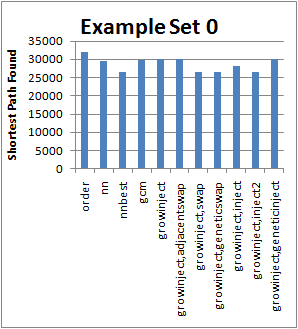
\includegraphics[totalheight=0.27\textheight]{set0.png}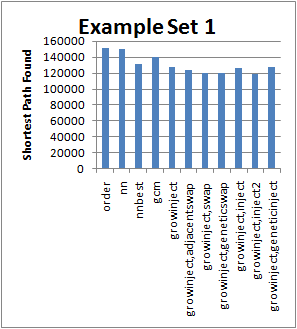
\includegraphics[totalheight=0.27\textheight]{set1.png}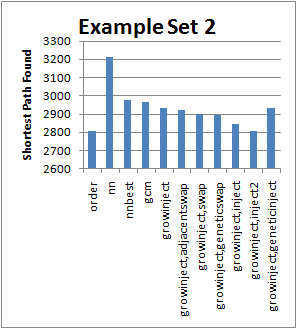
\includegraphics[totalheight=0.27\textheight]{set2.png}

\section*{Sources}

\end{document}
